\chapter{\RU{Файл для сохранения состояния в игре Millenium}\EN{Millenium game save file}}

\RU{Игра}\EN{The} ``Millenium Return to Earth'' \RU{под DOS довольно древняя (1991 или 1992), позволяющая
добывать ресурсы, строить корабли, снаряжать их на другие планеты, итд}\EN{is an ancient DOS game (1991 or 
1992), allowing to mine resources, build ships,
equip them to other planets, and so on}\footnote{\RU{Её можно скачать бесплатно}\EN{It can be downloaded for free}
\href{http://thehouseofgames.org/index.php?t=10&id=110}{\RU{здесь}\EN{here}}}.

\RU{Как и многие другие игры, она позволяет сохранять состояние игры в файл.}
\EN{Like many other games, it allows to save all game state into file.}

\RU{Посмотрим, сможем ли мы найти что-нибудь в нем}\EN{Let's see, if we can find something in it}.

\RU{В игре есть шахта}\EN{So there is a mine in the game}.
\RU{Шахты на некоторых планетах работают быстрее, на некоторых других --- медленнее}\EN{Mines at some planets 
work faster, or slower on another}. 
\RU{Набор ресурсов также разный}\EN{Resource set is also different}.

\RU{Здесь видно, какие ресурсы добыты в этот момент}\EN{Here I see what resources are mined at the time}: 
\figref{fig:mill_1}.
\RU{Я сохранил состояние игры}\EN{I save a game state}.
\RU{Это файл размером}\EN{This is a file of size} 9538 \RU{байт}\EN{bytes}.

\RU{Я подождал несколько ``дней'' здесь в игре и теперь в шахте добыто больше ресурсов}\EN{I wait some 
``days'' here in game, and now we've got more resources at the mine}: \figref{fig:mill_2}.
\RU{Я снова сохранил состояние игры}\EN{I saved game state again}.

\RU{Теперь просто попробуем сравнить оба файла побайтово используя простую утилиту FC под DOS/Windows:}
\EN{Now let's try just to do binary comparison of the save files using simple DOS/Windows FC utility:}

\lstinputlisting{ff/millenium/fc_result.txt}

\RU{Вывод здесь неполный, там было больше отличий, но я обрезал результат до самого интересного.}
\EN{The output is unfull here, there are more differences, but I cut result to the most interesting.}

\RU{В первой версии было 14 единиц водорода (hydrogen) и 102 --- кислорода (oxygen).}
\EN{At first state, I have 14 ``units'' of hydrogen and 102 ``units'' of oxygen.}
\RU{Во второй версии 22 и 155 единиц соответственно.}
\EN{I have 22 and 155 ``units'' respectively at the second state.}
\RU{Если эти значения сохраняются в файл, мы должны увидеть разницу}\EN{If these values are saved into 
save-file, we should see this in difference}.
\RU{И она действительно есть}\EN{And indeed so}. 
\RU{Там}\EN{There are} 0x0E (14) \RU{на позиции}\EN{at} 0xBDE \RU{и это значение}\EN{position and this value is} 
0x16 (22) \RU{в новой версии файла}\EN{in new version of file}.
\RU{Это наверное водород}\EN{This could be for hydrogen}.
\RU{Там также}\EN{There is} 0x66 (102) \RU{на позиции}\EN{at position} 0xBDC \RU{в старой версии и}\EN{in old 
version and} 0x9B (155) \RU{в новой версии файла}\EN{in new version of file}. 
\RU{Это наверное кислород}\EN{This could be for oxygen}.

\RU{Я выложил обе версии файла на своем сайте для тех кто хочет их изучить 
(или поэкспериментировать)}\EN{There both of files I put on my website for those who wants to inspect them 
(or experiment) more}: \url{http://beginners.re/examples/millenium_DOS_game/}.

\RU{Новую версию файла я открыл в Hiew и отметил значения, связанные с ресурсами добытыми на шахте в 
игре}\EN{Here is a new version of file opened in Hiew, I marked values related to resources mined in the game}: 
\figref{fig:mill_hiew3}.
\RU{Я проверил каждое, и это они}\EN{I checked each, and these are}.
\RU{Это явно 16-битные значения: не удивительно для 16-битной программы под DOS, где \Tint имел длину в 
16 бит.}
\EN{These are clearly 16-bit values: not a strange thing for DOS 16-bit software where \Tint has 16-bit width.}

\RU{Проверим наши предположения}\EN{Let's check our assumptions}.
\RU{Я записал}\EN{I'm writing} 1234 (0x4D2) \RU{на первой позиции (это должен быть водород)}\EN{value at 
first position (this should be hydrogen)}:
\figref{fig:mill_hiew4}.

\RU{Затем я загрузил измененный файл в игру и посмотрел на статистику в шахте}\EN{Then I loaded changed 
file into game and taking a look on mine statistics}: \figref{fig:mill_5}.
\RU{Так что да, это оно}\EN{So yes, this is it}.

\RU{Попробуем пройти игру как ожно быстрее, установим максимальные значения везде}\EN{Now let's try to 
finish the game as soon as possible, set maximal values everywhere}: \figref{fig:mill_hiew7}.

0xFFFF \RU{это}\EN{is} 65535, \RU{так что да, у нас много ресурсов теперь}\EN{so yes, we now have a 
lot of resources}: \figref{fig:mill_6}.

\RU{Я пропустил еще несколько ``дней'' в игре и оппа}\EN{I skipped some ``days'' in game and oops}! 
\RU{Некоторых ресурсов стало меньше}\EN{I have lower amount of some resources}: \figref{fig:mill_8}.
\RU{Это просто переполнение}\EN{That's just overflow}. 
\RU{Разработчик игры вероятно никогда не думал, что значения ресурсов будут такими большими,
так что, здесь наверное нет проверок на переполнение, но шахта в игре ``работает'', ресурсы добавляются,
отсюда и переполнение.}
\EN{Game developer probably didn't thought about such high amounts of resources,
so there are probably no overflow check, but mine is ``working'' in the games, resources are added,
hence overflow.}
\RU{Полагаю, я не должен был быть таким жадным}\EN{I shouldn't be that greedy, I suppose}.

\RU{Здесь наверняка еще какие-то значения в этом файле}\EN{There are probably a lot of more values 
saved in this file}.

\RU{Так что это очень простой способ читинга в играх}\EN{So this is very simple method of cheating in games}.
\RU{Файл с таблицей очков также можно легко модифицировать}\EN{High score files are often can be easily 
patched like that}.

\begin{figure}[H]
\centering
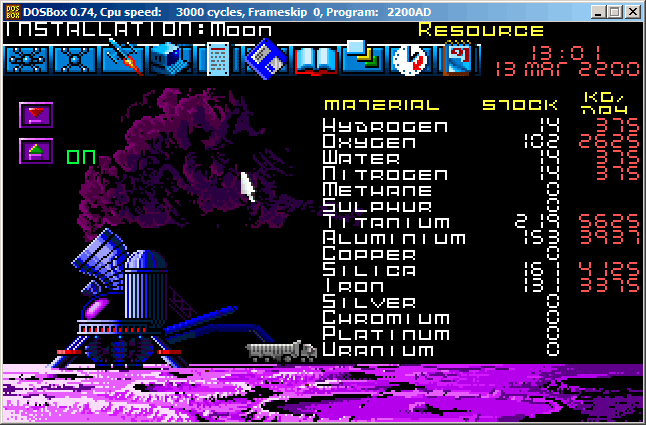
\includegraphics[scale=\FigScale]{ff/millenium/1.png}
\caption{\RU{Шахта: первое состояние}\EN{Mine: state 1}}
\label{fig:mill_1}
\end{figure}

\begin{figure}[H]
\centering
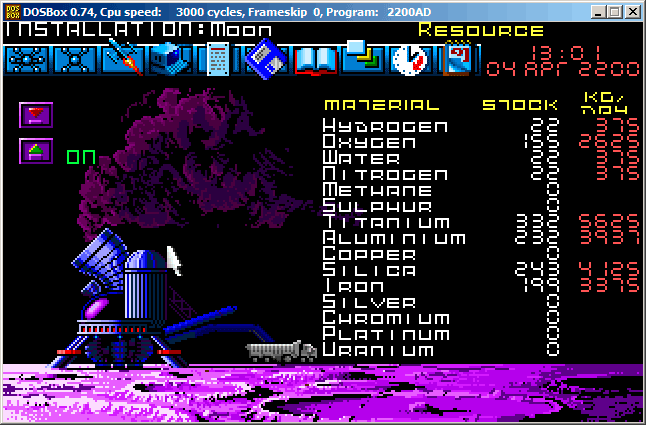
\includegraphics[scale=\FigScale]{ff/millenium/2.png}
\caption{\RU{Шахта: второе состояние}\EN{Mine: state 2}}
\label{fig:mill_2}
\end{figure}

\begin{figure}[H]
\centering
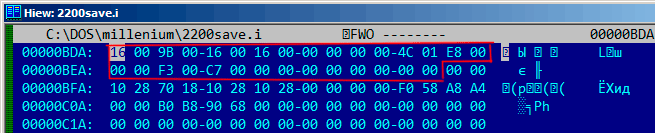
\includegraphics[scale=\FigScale]{ff/millenium/hiew3.png}
\caption{Hiew: \RU{первое состояние}\EN{state 1}}
\label{fig:mill_hiew3}
\end{figure}

\begin{figure}[H]
\centering
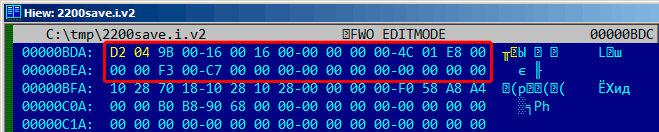
\includegraphics[scale=\FigScale]{ff/millenium/hiew4.png}
\caption{Hiew: \RU{запишем там}\EN{let's write 1234} (0x4D2)\EN{ there}}
\label{fig:mill_hiew4}
\end{figure}

\begin{figure}[H]
\centering
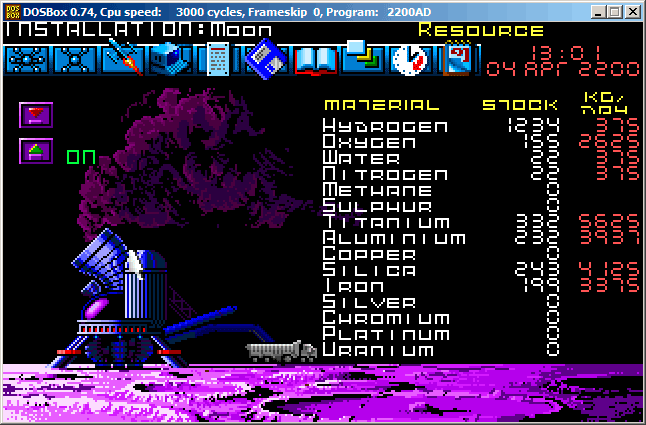
\includegraphics[scale=\FigScale]{ff/millenium/5.png}
\caption{\RU{Проверим значение водорода}\EN{Let's check for hydrogen value}}
\label{fig:mill_5}
\end{figure}

\begin{figure}[H]
\centering
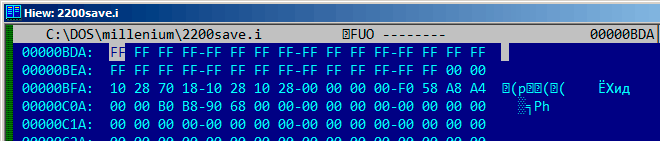
\includegraphics[scale=\FigScale]{ff/millenium/hiew7.png}
\caption{Hiew: \RU{установим максимальные значения}\EN{let's set maximal values}}
\label{fig:mill_hiew7}
\end{figure}

\begin{figure}[H]
\centering
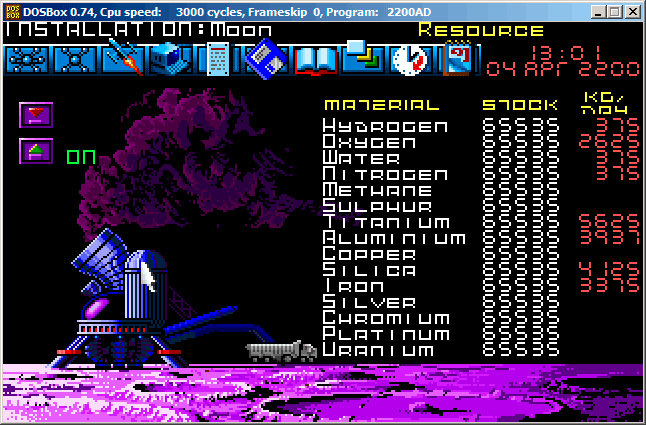
\includegraphics[scale=\FigScale]{ff/millenium/6.png}
\caption{\RU{Все ресурсы теперь действительно}\EN{All resources are} 65535 (0xFFFF)\EN{ indeed}}
\label{fig:mill_6}
\end{figure}

\begin{figure}[H]
\centering
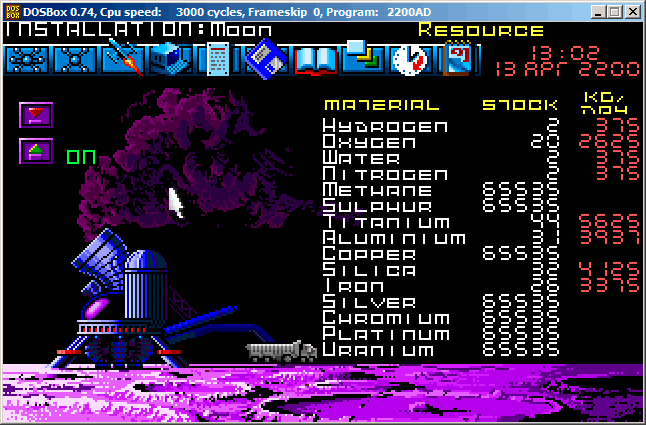
\includegraphics[scale=\FigScale]{ff/millenium/8.png}
\caption{\RU{Переполнение переменных ресурсов}\EN{Resource variables overflow}}
\label{fig:mill_8}
\end{figure}
